\documentclass[bigtut]{tutorial}\usepackage[]{graphicx}\usepackage[]{color}
%% maxwidth is the original width if it is less than linewidth
%% otherwise use linewidth (to make sure the graphics do not exceed the margin)
\makeatletter
\def\maxwidth{ %
  \ifdim\Gin@nat@width>\linewidth
    \linewidth
  \else
    \Gin@nat@width
  \fi
}
\makeatother

\definecolor{fgcolor}{rgb}{0.345, 0.345, 0.345}
\newcommand{\hlnum}[1]{\textcolor[rgb]{0.686,0.059,0.569}{#1}}%
\newcommand{\hlstr}[1]{\textcolor[rgb]{0.192,0.494,0.8}{#1}}%
\newcommand{\hlcom}[1]{\textcolor[rgb]{0.678,0.584,0.686}{\textit{#1}}}%
\newcommand{\hlopt}[1]{\textcolor[rgb]{0,0,0}{#1}}%
\newcommand{\hlstd}[1]{\textcolor[rgb]{0.345,0.345,0.345}{#1}}%
\newcommand{\hlkwa}[1]{\textcolor[rgb]{0.161,0.373,0.58}{\textbf{#1}}}%
\newcommand{\hlkwb}[1]{\textcolor[rgb]{0.69,0.353,0.396}{#1}}%
\newcommand{\hlkwc}[1]{\textcolor[rgb]{0.333,0.667,0.333}{#1}}%
\newcommand{\hlkwd}[1]{\textcolor[rgb]{0.737,0.353,0.396}{\textbf{#1}}}%

\usepackage{framed}
\makeatletter
\newenvironment{kframe}{%
 \def\at@end@of@kframe{}%
 \ifinner\ifhmode%
  \def\at@end@of@kframe{\end{minipage}}%
  \begin{minipage}{\columnwidth}%
 \fi\fi%
 \def\FrameCommand##1{\hskip\@totalleftmargin \hskip-\fboxsep
 \colorbox{shadecolor}{##1}\hskip-\fboxsep
     % There is no \\@totalrightmargin, so:
     \hskip-\linewidth \hskip-\@totalleftmargin \hskip\columnwidth}%
 \MakeFramed {\advance\hsize-\width
   \@totalleftmargin\z@ \linewidth\hsize
   \@setminipage}}%
 {\par\unskip\endMakeFramed%
 \at@end@of@kframe}
\makeatother

\definecolor{shadecolor}{rgb}{.97, .97, .97}
\definecolor{messagecolor}{rgb}{0, 0, 0}
\definecolor{warningcolor}{rgb}{1, 0, 1}
\definecolor{errorcolor}{rgb}{1, 0, 0}
\newenvironment{knitrout}{}{} % an empty environment to be redefined in TeX

\usepackage{alltt}
\unitcode{MATH1005}
        \unitname{Statistics}
        \semester{Summer/Winter/Semester2}
        \sheetnumber2


\usepackage{graphicx}
\withsolutions
\IfFileExists{upquote.sty}{\usepackage{upquote}}{}
\begin{document}
\lettersfirst

\begin{tutorial}

The aim of this tutorial is to introduce you to the framework of problem solving in hypothesis testing, before using the formal tests (Topics 9-12).

\begin{questions}

\question Hypothesis Testing \\

`The (null hypothesis) is ... never proved or established, but is possibly disproved, in the context of experimentation. Every experiment may be said to exist only in order to give the facts a chance of disproving the null hypothesis.' (Ronald Fisher, Design of Experiments, 1935, p19). \\

Summarise this quote in your own words.

\question
It is known that the mean Brinell hardness of ductile iron pieces is 170 units.  An engineer believes that it has increased.  He measures the Brinell hardness of 25 pieces of ductile iron that were subcritically annealed, resulting in the following data: \\

170  167	174	179	179 156	163	156	187	156 183	179	174	179	170 156 187	179	183	174 187	167	159	170	179 \\

\begin{knitrout}
\definecolor{shadecolor}{rgb}{0.969, 0.969, 0.969}\color{fgcolor}\begin{kframe}
\begin{alltt}
\hlstd{x}\hlkwb{=}\hlkwd{c}\hlstd{(}\hlnum{170}\hlstd{,}\hlnum{167}\hlstd{,}\hlnum{174}\hlstd{,}\hlnum{179}\hlstd{,}\hlnum{179}\hlstd{,}\hlnum{156}\hlstd{,}\hlnum{163}\hlstd{,}\hlnum{156}\hlstd{,}\hlnum{187}\hlstd{,}\hlnum{156}\hlstd{,}\hlnum{183}\hlstd{,}\hlnum{179}\hlstd{,}\hlnum{174}\hlstd{,}\hlnum{179}\hlstd{,}\hlnum{170}\hlstd{,}\hlnum{156}\hlstd{,}
    \hlnum{187}\hlstd{,}\hlnum{179}\hlstd{,}\hlnum{183}\hlstd{,}\hlnum{174}\hlstd{,}\hlnum{187}\hlstd{,}\hlnum{167}\hlstd{,}\hlnum{159}\hlstd{,}\hlnum{170}\hlstd{,}\hlnum{179}\hlstd{)}
\end{alltt}
\end{kframe}
\end{knitrout}

\begin{parts}
\part Write down the hypotheses, defining all symbols. \\

\part Summarise the data.

\begin{knitrout}
\definecolor{shadecolor}{rgb}{0.969, 0.969, 0.969}\color{fgcolor}\begin{kframe}
\begin{alltt}
\hlkwd{mean}\hlstd{(x)}
\hlkwd{sd}\hlstd{(x)}
\hlkwd{fivenum}\hlstd{(x)}
\hlkwd{hist}\hlstd{(x)}
\end{alltt}
\end{kframe}
\end{knitrout}

\vspace{.5cm}
\part What information about the sample best relates to the hypotheses? From the sample, what would you infer about the hypotheses? 
\end{parts}

\begin{solution}

Let $\mu$ be the mean Brinell hardness of ductile iron pieces.
$H_{0}: \mu = 170$ vs $H_{1}: \mu > 170$. \\

The mean of the sample would be the best guess to mean of population, as specified in hypotheses. As  $\bar{x}= 172.52$, we might first infer that the data supports $H_{1}$ rather than $H_{0}$. However, we need to also consider the relatively large standard deviation of $s \approx 10.31$.
\end{solution}




\question
A biologist is interested in determining whether seedlings treated with fertiliser result in more yield. The standard height is 16 cm. A random sample of 32 seedlings treated with fertiliser results in the following yields: \\

11.5  11.8	15.7	16.1	14.1	10.5 15.2	19.0	12.8	12.4	19.2	13.5 16.5	13.5	14.4	16.7	10.9	13.0 15.1	17.1	13.3	12.4	8.5	14.3 12.9	11.1	15.0	13.3	15.8	13.5 9.3	12.2		 \\ 	 

Is there evidence that the fertiliser has worked?

\begin{knitrout}
\definecolor{shadecolor}{rgb}{0.969, 0.969, 0.969}\color{fgcolor}\begin{kframe}
\begin{alltt}
\hlstd{x}\hlkwb{=}\hlkwd{c}\hlstd{(}\hlnum{11.5}\hlstd{,}\hlnum{11.8}\hlstd{,}\hlnum{15.7}\hlstd{,}\hlnum{16.1}\hlstd{,}\hlnum{14.1}\hlstd{,}\hlnum{10.5}\hlstd{,}\hlnum{15.2}\hlstd{,}\hlnum{19.0}\hlstd{,}\hlnum{12.8}\hlstd{,}\hlnum{12.4}\hlstd{,}\hlnum{19.2}\hlstd{,}\hlnum{13.5}\hlstd{,}\hlnum{16.5}\hlstd{,}\hlnum{13.5}\hlstd{,}
      \hlnum{14.4}\hlstd{,}\hlnum{16.7}\hlstd{,}\hlnum{10.9}\hlstd{,}\hlnum{13.0}\hlstd{,}\hlnum{15.1}\hlstd{,}\hlnum{17.1}\hlstd{,}\hlnum{13.3}\hlstd{,}\hlnum{12.4}\hlstd{,}\hlnum{8.5}\hlstd{,}\hlnum{14.3}\hlstd{,}\hlnum{12.9}\hlstd{,}\hlnum{11.1}\hlstd{,}\hlnum{15.0}\hlstd{,}\hlnum{13.3}\hlstd{,}\hlnum{15.8}\hlstd{,}
      \hlnum{13.5}\hlstd{,}\hlnum{9.3}\hlstd{,}\hlnum{12.2}\hlstd{)}
\hlkwd{mean}\hlstd{(x)}
\hlkwd{var}\hlstd{(x)}
\hlkwd{sd}\hlstd{(x)}
\hlkwd{hist}\hlstd{(x)}
\end{alltt}
\end{kframe}
\end{knitrout}

\begin{solution}

Let $\mu$ be the mean yield of the seedings.
We could propose: $H_{0}: \mu = 16$ vs $H_{1}: \mu > 16$. \\

The sample results in:  $\bar{x} \approx 13.77$ with $sd \approx 2.51$.
The data appears to be consistent with $H_{0}$, compared to $H_{1}$.
\end{solution}

\question
An investment advisor offers you a monthly income investment scheme which promises a variable return each month. 
For the past  2 years, the scheme has returned an average of \$180 per month, with a  standard deviation of \$75.
You only want to invest in the scheme if you can get an average of a \$190 monthly income. Should you invest in this scheme?

\begin{solution}
Let $\mu$ be the mean monthly return of scheme.
We propose: $H_{0}: \mu = 190$ (return wanted) vs $H_{1}: \mu \neq 190$. \\

The sample results in:  $\bar{x} \approx 180$ with $sd \approx 75$.  Investment could result in both big returns or big losses. How would you decide?

\end{solution}

\question
An international study was investigating the connection between breast cancer and age of mother for first pregnancy. Women with breast cancer were identified in selected hospitals in the United States, Greece, Yugoslavia, Brazil, and Japan. Women of similar age, without breast cancer, were chosen from each hospital, to be the control. \\

The women were divided into 2 categories, based on their age at first birth:

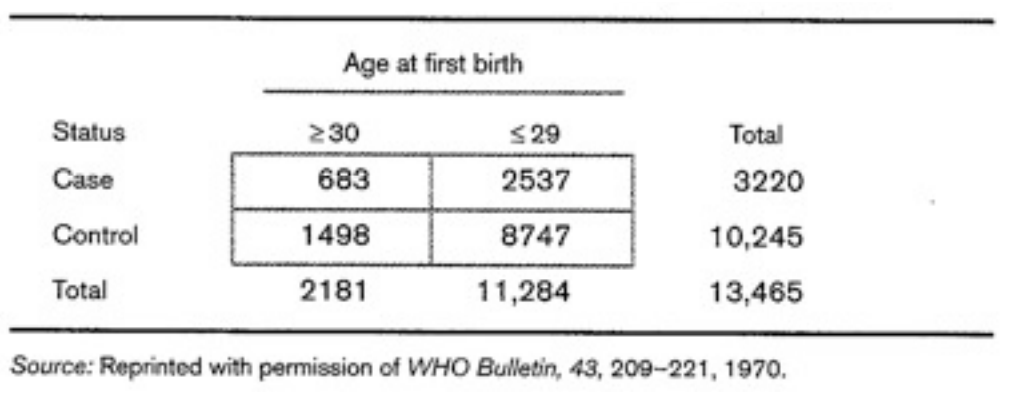
\includegraphics[scale=0.5]{DataBreastCancer.jpg}

Set up appropriate hypotheses. What does the data suggest?

\begin{solution} 

Let $p_{1}$ be the probability that age at first birth is $ \geq 30$
in the women with breast cancer. \\
Let $p_{2}$ be the probability that age at first birth is $\geq
30$ in control women. \\

$H_{0}: p_{1} - p_{2} = 0$ vs $H_{1}: p_{1} - p_{2} \neq 0$.

\end{solution}



\end{questions}
\end{tutorial}
\end{document}



\end{document}

